\documentclass[a4paper,10pt]{article}
\usepackage[utf8x]{inputenc}
\usepackage{graphicx}

%opening
\title{Spam Classification \& Spam Filtering}
\author{Girish Sastry}

\begin{document}

\maketitle

\begin{abstract}

Spam is a concept that has been around a long time. These unsolicited messages dilute the message pool, causing
frustration and leading to unhappy consumers. With the advent of the internet and electronic mail, the the barrier
to entry for spamming has become very low. Recipients of spam e-mail messages must waste time and effort to delete
irrelevant spam e-mails. This paper focuses on the analysis of different methods for spam classification. We compare
the learning performance of different types of classifiers on the SpamBase e-mail data set. We also look at different tools and programming languages
to express these machine learning computations. We conclude by discussing the tradeoffs of our different methods and
our tools, and point to the results we learned by applying these machine learning methods to the SpamBase data set.

\end{abstract}

\section{Introduction}
\subsection{Spam}

In today's digital age, concern about the reception of unsolicited junk e-mail, (``Spam''), has been increasing.
When spam e-mail is received in small quantities, it may not be a hassle for users to manually delete unwanted
e-mails. However, because the barrier of entry for spammers is so low for e-mail, users would have to spend a lot
of time and resources to keep their inboxes clean and void of spam. For many internet companies whose business
models are based on advertising, spam is the invisible nemesis that sucks away advertising money. For example, 
companies such as Facebook, Google, and Twitter, all make more money based on advertisement impressions. The
more time a user spends on these sites, the more likely they will be to click an ad. The prescence of spam 
reduces this and presents many data curation issues. Thus, spam filtering is an important problem in today's
internet age.

How do we recognize a spam e-mail? There are many features present in the body of th e-mail message that may
indicate spam. In a 1998 study, authors reported the different purposes of reported spam e-mails[1]:

 \begin{figure}[h]
 \centering
 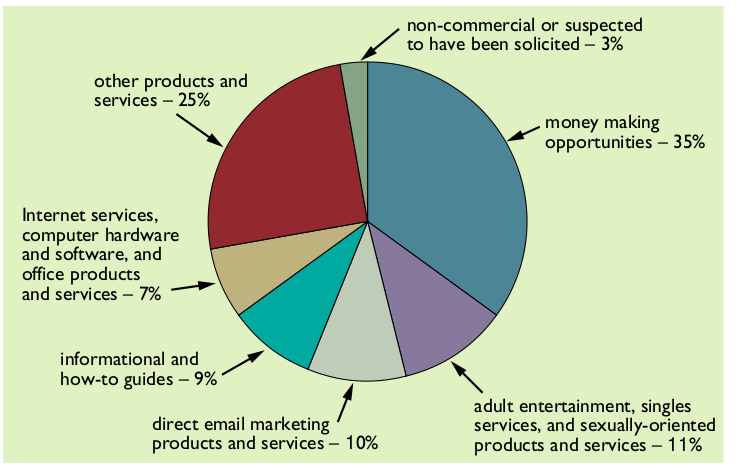
\includegraphics[width=100mm]{../resources/spam-pi-chart.png}
 % spam-pi-chart.png: 738x468 pixel, 72dpi, 26.03x16.51 cm, bb=0 0 738 468
 \caption{Type of products advertised by spam e-mails}
\end{figure}

Similar to the telemarketers of old, spam e-mails want to sell stuff to users. Recognizing this from the features
present in the body of an e-mail is hard, as these features are probably not globally constant -- they would vary
not only from spammer to spammer, but from user to user. One man's gold may be another man's trash. Thus, in practice,
spam filtering must be robust globally, but also personalized to a user's specific needs.

\subsection{SpamBase Data Set}

The SpamBase data set, available for free from the UCI Machine Learning repository, was used for spam classification
for this project. The SpamBase data set was collected internally by Hewlett Packard Labs for research purposes and
then released to the public. The spam emails were self-reported as being spam. While spam for one e-mail user may
not be spam for another, the data set attempts to extract some relevant features in order to make this a machine
learning problem. There are fifty-five features total. Forty-eight of these features are continuous, real-valued
attributes for word frequencies. Six are continuous, real-valued attributes for character frequencies. The rest 
of the features take into account other commonly seen features in spam: excessively long capitalized strings. Figure 2
shows a scatterplot matrix of the first five features in the data set. It is important to note that due to the nature
of the data set, we will not see strong correlations immediately present. There is a wide variance in the features for
spam emails -- once again, one person's spam is another person's coupon.

\begin{figure}[h]
 \centering
 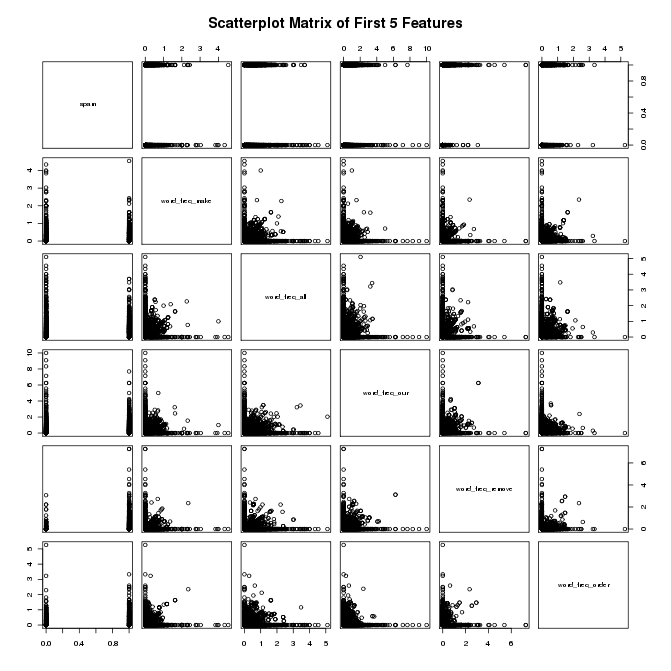
\includegraphics[width=100mm]{../resources/scatter-plot-5.png}
 % scatter-plot-5.png: 671x671 pixel, 72dpi, 23.67x23.67 cm, bb=0 0 671 671
 \caption{Scatter plot matrix of first 5 features from SpamBase}
\end{figure}

\subsection{Goals}

For this project, we have two overall goals.

\subsubsection{Classification Performance}

First, we would like to measure and compare the classification performance of a number of methods. These include
methods discussed in class and out of class. For this project, we consider:

\begin{itemize}
 \item Decision Trees
 \item k-Nearest Neighbor
\end{itemize}

We would like to minimize both misclassification error and false positives. In the case of spam, false positives
very bad.

\subsubsection{Tools to Express Computations}

Next, we would like to explore the different tools available to express these computations. For most of the course
we have been using R, the ``statistical programming language.'' However, there are some limitations of R that 
may not make it the best tool for the task. For example, R's data frame's are stored in memory. This means that
R is not suited for large data sets that do not fit in memory. With today's petabytes and petabytes of data being
produced on the web, it is time to consider other tools. For this project, we use the following programming languages
and toolkits:

\begin{itemize}
 \item WEKA Toolkit (Java)
 \item Clojure
 \item R
\end{itemize}

Clojure is a dialect of Lisp, and has recently exploded in popularity. There have been several machine learning
packages written in Clojure. The appeal of Clojure as a general purpose programming language is quite clear.
It is a Lisp, so we obtain all the benefits of a dynamically typed, functional programming language with minimal syntax.
This means that computations can be expressed more succinctly than canonical imperative programming languages like
C or Java. Functions are passed around as values, so, just as in mathematics, functions can be composed and passed
as arguments to functions.

For statistical computing, Lisp has recently drawn speculation as the next big thing, and as R's successor[4]. R's limitations
include:

\begin{itemize}
 \item Pass-by-value computations: only local values of parameters are modified
 \item Scalar operations: Vectorized operations execute much faster than scalar operations, but are harder to implement
   \item Native code compilation: R is slow. Thus, in many intensive use cases, the performance-critical code is moved to C.
 \item Rudimentary type system: Type checking, inference, and analysis is a real workhorse of the compiler, and can aid the programmer
 in debugging. R lacks this. [4]
\end{itemize}

Clojure is a Lisp that operates on the Java Virtual Machine, which means that it has access to the huge assortment of Java
libraries. This makes it an ideal candidate for a new ``tool'' to experiment with in this project.

\section{Results \& Discussion}

\subsection{k-Nearest Neighbors}

The k-Nearest Neighbors classification algorithm is one of the simplest classification algorithms. Indeed, it is the first algorithm,
other than univariate regression, that we covered in this course. k-Nearest Neighbors attempts to classify an object by its nearest
neighbors in the feature space. An object is classified by a majority vote of its neighbors. If $k$ is small, say 1, then an object
``takes on'' the properties of its nearest neighbor. 

The distance metric used to find the ``nearest'' neighbor is usually the Euclidean distance metric, and this is what is used in our
experiments. For some classification problems in information retrieval and text classification, other distance metrics, such as
Hamming Distance, may be used[3].

It is up to the experimenter to set the value of $k$ in the k-Nearest Neighbors algorithm. There a couple things to consider when
setting this value. An extremely low value of $k$ is extremely succeptible to noise or irrelevant, less important features in the
data set. Intuitively, for the SpamBase data set, this could be something like \texttt{char\_freq\_(}, where it is not immediately clear
what sort of correlation this could have with spam or non-spam emails. We go through 10-fold cross validation to choose the optimal
value of $k$ for SpamBase classification -- in our case, $k=5$.

One drawback to the majority voting that is present in the k-Nearest Neighbors algorithm is that classes that tend to appear more
frequently in the data set (i.e. more instances) also tend to dominate the classification results. In our case, more than 50\% of the
SpamBase data set is ``non-spam'' e-mails, so we may see this domination.


\subsection{Naive Bayes}

Next, we run a Naive Bayesian classifier on the SpamBase data set. Naive bayes classifiers are computationally very fast, relatively
easy to implement, and relatively easy to understand. In addition, and perhaps in spite of their simplicity, Naive Bayes classifiers have
worked pretty well in practice[6].These attributes make Naive Bayes classifiers a prime classifier choice for this 
set of experiments.

Naive bayes classifiers are simple probabilistic based on Bayes' Theorem. The ``naive'' in Naive Bayes refers to the strong independence
assumption inherent in these classifiers -- each feature is assumed to be independent of other features. Assuming $n$ features ranging
from $F_1,F_2,...,F_n$, and a class variable called $C$, there are a few inputs to the probability model:
\begin{itemize}
 \item Prior probabilities: $P(C)$
   \item Likelihood: $P(F_1,..,F_n)|C$
   \item Evidence: $P(F_1,...,F_n)$
\end{itemize}

And we can write, using Bayes Theorem, the formula to calculate the posterior probability:

 $$ P(C|F_1,...,F_n) = \frac{P(C)P(F_1,...,F_n|C}{P(F_1...F_n} $$
 
In practice, the ``evidence'' probability is usually a constant, since it doesn't depend on the class variable, $C$.

There a couple reasons why the assumption of independence is an ok assumption. First, we just need the relative probabilities 
in order to make an accurate prediction. These relative proabilities just need to be ranked correctly. We do not need the extra
information regarding class probabilities. This implies that Naive Bayes is a pretty robust classification method. Second, variable 
decoupling has some positive side-effects. Variable decoupling reduces higher order interaction terms that take away from the
predictive model and thus helps reduce the curse of dimensionality. Thus, the ``naive'' assumption of strong independence that is
present in the model is not as naive as it initially seems.

The overall classification model is as follows[7]: 

\begin{figure}[h]
 \centering
 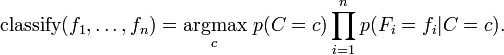
\includegraphics[width=100mm]{../resources/bayes-classify-formula.png}
 % bayes-classify-formula.png: 504x55 pixel, 72dpi, 17.78x1.94 cm, bb=0 0 504 55
 \caption{Classification model for Naive Bayes}
\end{figure}


We obtain a training error of 10.60\% and a test error of 10.43\% using the Naive Bayes classifier. This misclassification
error is not that good. It appears that the assumptions that Naive Bayes makes, the very ones that we argued were ok
assumptions to make, skew the results. We also tried two other Naive Bayes algorithms from the WEKA machine learning
toolkit and obtained similar results. \texttt{ComplementNaiveBayes} provided a slightly better result of 9.14\% training
error and 9.58\% test error. While better, this is still not the best error we could get.

\subsection{Support Vector Machines}

Support vector machine is a an interesting learning method that is a non-probabilistic binary classifier. They work by
predicting for each instance of data the class that the data is a part of.

The model that a support vector machine builds works as follows: the suppoer vector machine constructs a hyperplane 
(or a set of hyperplanes for a higher dimensional space). This hyperplane that is drawn can be described by the
characteristic equation:

$$ \textbf{w} \textbf{x} + b = 0 $$

 where 
\begin{itemize}
 \item $\textbf{w}$ is normal to the hyperplane,
   \item $\frac{b}{||\textbf{w}||}$ is the distance from the origin to the hyperplane
\end{itemize}

The term ``support vector'' refers to the vectors, or instances of data, that are closest to the hyperplane. The goal of
support vector machines is to orient the hyperplane so that the supper vectors are as far as possible from the hyperplane.

\begin{figure}[h]
 \centering
 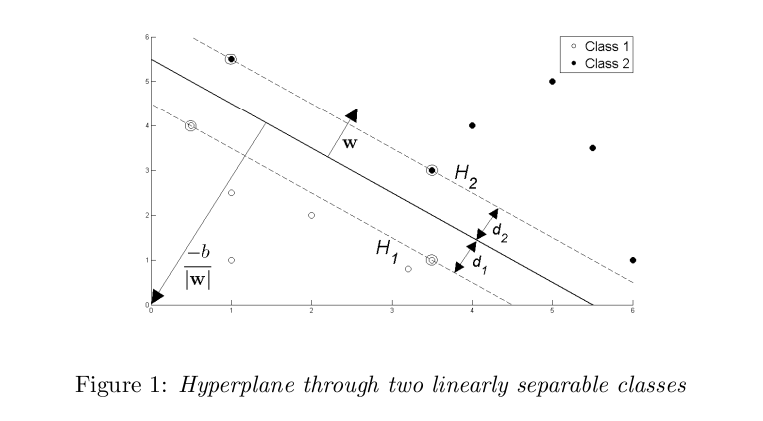
\includegraphics[width=100mm]{../resources/svm-example.png}
 % svm-example.png: 763x421 pixel, 72dpi, 26.92x14.85 cm, bb=0 0 763 421
 \caption{Support vectors \& hyperplane for two classes, example}
\end{figure}

Thus, support vector machines attempt to assign values to $\textbf{w}$ and $b$ for the data set.

It should be noted that this theoretical model of support vector machines assumes that the data is linearly separable into 
two classes. To deal with data that is not fully linearly separable, the model relaxes some of the optimization constraints
when choosing values for $\textbf{w}$ and $b$[2].

On the spam data set, we obtain a training error of 6.50\% and a teset error of 6.38\%. This is a decent result, and beats
the 7\% error that is considered ``good.'' This better performance can be explained by some of the advantages of support
vector machines. Support vector machines often perform better when the data set is small and noisy. This is the case with
the SpamBase data set. We have a relatively small number of instances. The data set is noisy because of the nature of spam.
One person may report something with \texttt{word\_freq\_hp} as spam, while it is not to another person.


\subsection{Decision Trees}

First, we consider decision trees. Decision trees are a simple procedure that classifies instances of data. They work by
constructing a tree of decisions, where the leaf nodes represent classifications, and each intermediate node represents
a decision based on a conjunction of features that leads to a classification.

Using unpruned decision trees, we obtain a training error of 10.53\% and a test error of 9.98\%.

Next, we turn an ensemble method of classification using decision trees. We use boosting on the SpamBase data set.
Boosting is based on the simple question: ``Can a set of weak learners create a single strong learner?''[5] Boosting
works, in the general case, by iteratively learning weak classifiers and then weighting and adding them to a final strong
classifier. While there are many algorithms for boosting, we use Adaboost here. Boosting seeks to minimize the convex
loss function

$$ \sum_i e^{-y_i f(x_i)} $$

while seeking a function 

$$ f = \sum_t \alpha_t h_t $$

On the SpamBase data set, boosting gives a training error of 5.00\% and a test error of 5.15\%. This is much better
than any of the other methods so far. This is probably due to the ensemble method of classification. At a high level,
AdaBoost minimizes the exponential loss function. Thus, it basically chooses a hyperplane and orients it away from
the two classes, in a similar way to support vector machines. It seems that based on these results that ensemble methods
are the way to go. To further test this, we look at support vector machines next.

Next, we turn to another ensemble method of classification using decision trees. Random Forests are a way of using a slightly perturbed
version of the data set in simulation along with multiple decision trees to classify data. Random forests combine the idea of
``bagging'' and random feature selection to produce multiple decision trees under controlled variation. The learning algorithm
is as follows[3]:

\begin{enumerate}
  \item Init: Let $N$ be the number of instances in training set, and the number of features be $M$
  \item We know $m$ input variables which are used to determine the decision at each node of the tree. $m << M$.
  \item Choose a training set: Choose $N$ times with replacement from all $N$ training instances
    \item For each node in the tree, randomly choose $m$ variables used to make the decision at that point. 
    \item Let each tree grow and do not prune
\end{enumerate}

We obtain a training set error of 4.79\% and a test set error of 4.69\%. The confusion matrices for both the training and test
sets are reported as follows:

Our training and test error rates are very good. They beat the ``good'' error rates by almost half. The number of false positives
did not vary that much from our other tree based results, but there are still false positives. It seems that random forests, and perhaps
ensemble methods in general, do much better at predicting spam. Because of possible high inter-variable correlation that many of
other methods do not account, random forests perform better.
\section{Discussion}

It is interesting to note that Naive Bayes did not provide us with good results. In the Computer Science field, most companies that
use spam filters in production use Naive Bayes as the workhorse of their spam filters. It is evident, based on our results here, and intuition,
that these same institutions also use ensemble methods for classification. An untuned Naive Bayes algorithm does not provide good results,
but the ensemble methods of random forests and AdaBoost do. Thus, it makes sense that spam filters in production use some combination of
learners on top Naive Bayes to implement their spam filters.

We experimented with different tools of Clojure, WEKA, and R in this project. We find that Clojure has probably the most potential to
write real machine learning systems. It is a very well designed language with many features and operates on the JVM. However, the current
landscape of machine learning libraries is very sparse. R just completely wins this category with easily obtainable packages from CRAN and 
other repositories. The syntax and semantic constructs of Clojure are very nice. It is very easy to compose your own functions and build up
in a modular style.

For all methods used, forcing a value of zero false-positives raises the training and test errors to 22\%-25\%. It seems hard to balance
the two factors of minimizing false-positives and misclassification error.

\section{Conclusions}

We conclude that ensemble methods for classification provide better results than singular methods for classification. We also conclude
that real production spam filters are produced by some variation of ensemble methods. It seems that Naive Bayes alone is very bad, but perhaps
combined with other methods it improves drastically. 

\bibliographystyle{plain}

\nocite{Lotte_topicalreview, kearns, spam!, lisp, fletcher, hastie01statisticallearning, bayes}

\bibliography{references}

\section{Appendix}

\end{document}
